\documentclass{sig-alternate}
\usepackage[latin1]{inputenc}
\usepackage{graphicx}
\usepackage{url}

\begin{document}

\conferenceinfo{GECCO'15 Student Workshop,} {July 11-15, 2015, Madrid, Spain.}
\CopyrightYear{2015}
\crdata{TBA}
\clubpenalty=10000
\widowpenalty = 10000

\title{Soft computing techniques applied to corporate and personal security}

\numberofauthors{1}
\author{
\alignauthor
P. de las Cuevas\\
\affaddr{Dept. of Computer Architecture}\\
\affaddr{and Computer Technology}\\
\affaddr{University of Granada, Spain}\\
\email{paloma@geneura.ugr.es}
}

\maketitle

\begin{abstract}
%What problem do you want to solve? Why do you want to solve it? Why
%do you think the techniques and methodology you're applying will
%solve it? Those are the three questions that you have to answer in an
%abstract - JJ
% Paloma - esto es b�sicamente porque el abstract est� cogido del resumen de lo del doctorado, para poder empezar por alguna cosa. Lo reescribo.

Inside a ``Bring Your Own Device'' environment, the employees can freely use their devices. This allows them mix their personal and work life, but at the same time, if the users are not aware of a risky situation, or that situation is not covered by a security policy or rule, this environment can become very insecure. % <- problem
The aim of this paper is defining a novel system architecture able to self-adapt itself, in the sense that it will learn from the past non secure situations, and therefore will be able to determine whether a new situation is risky or not. % <- solution
This system proposes the use of a variety of techniques, from Data Mining analysis of big amounts of recorded data, to Evolutionary Algorithms for refining a set of existing policies, maybe creating new ones. % <- solution, details
A preliminary study about the refinement of lists of permitted or non permitted URL connections helps to demonstrate that, by performing a good preprocessing of the data, useful conclusions can be extracted from new - unknown - situations. Therefore, it is possible to successfully extend a set of rules for covering new, and ponentially dangerous, situations. % <- why is possible
\end{abstract}

\category{H.4}{Information Systems Applications}{Miscellaneous}
\category{G.1.6}{Mathematics of Computing}{NUMERICAL ANALYSIS}[Optimization]

\terms{}

\keywords{Data Mining, Corporate Security Policies, Evolutionary Algorithms, Machine Learning, Classification}

%
%%%%%%%%%%%%%%%%%%%%%%%%%%%%%%% INTRODUCTION %%%%%%%%%%%%%%%%%%%%%%%%%%%%%%%
%
\section{Introduction}
\label{sec:intro}

The evolution from traditional mobile phones to the so-called
smartphones has changed the way people use their devices. In addition,
security threats have evolved too \cite{gangula2013survey}, so that
new security measures have to be adopted every time a new threat
appears. More concretely, smartphones have contributed to the creation
of a \textit{Bring Your Own Device} (BYOD) scenario in which people
use their own devices at work. Despite of all the advantages that this
environment might have, it is clear that this kind of situation
creates new security challenges for the Chief Security Officer (CSO)
of a company \cite{Opp_Security11}. This is because they want a fast response to any user action that might cause harm to the company, but without monitoring the users in a way that is against privacy. % because... the environment is
                                % not totally controlled, or
                                % controlled all the time, by the IT
                                % department of the company,
                                % because... - JJ
%Paloma - a�adido
The task of the CSO and the security department of a company, is establishing a list of security
measures to cope with all the security incidents which might happen in every environment,
so they build what is called a set of \textit{Corporate Security
  Policies} (CSPs). These are a set of security rules aiming at
% This happens only in BYOD environments? Also in normal
% company-issued phones or computers? How does that relate to BYOD?
% It might be obvious to you, but not to the average EC conference
% delegate - JJ
%Paloma - extendido
protecting company assets by defining permissions for every different
behaviour that could lead to security incidents
\cite{kaeo2003designing}. But when such companies embrace a constantly
changing environment, and allow their employees to use their own
devices, the risk of having security incidents grows, even if the
employees do not have intention of attacking the company
\cite{stanton2005analysis, breivik2002abstract}. Then, there is a need of constantly renew the CSPs, which it might be difficult if new threats appear without knowing it in advance (because they are not included in the security policies).

This paper proposes a system architecture, which should be easily
% this paper? Your thesis? Are you covering that whole topic in this
% paper? 
% Paloma - es verdad que no es el desarrollo en s�, lo he cambiado a que lo que se propone es la arquitectura
integrated in company servers, and capable of evolving the rules
included in a CSP by learning from past user behaviours which caused
security incidents. In order to achieve this, different techniques
% all past behaviours? Those that can be detected? - JJ
% Paloma - "those which caused security incidents", est� especificado, �crees que hace falta reescribir?
have to be applied. First, we assume that a company stores the
security incidents that have been produced, along with the context in
which they were produced. Context was defined by Abowd et
al. \cite{abowd1999towards} as ``any information that can be used to
characterize the situation of an entity''. Then, and given that this
means to analyse great quantities of data, Data Mining (DM) techniques
can help to extract useful information from it \cite{DeVel2001}, and
also from what can be considered as \textit{good behaviour} (this
means, actions that were permitted by the security rules). This
process would allow to build a classifier and to further classify new
situations. With the extracted conclusions from the performed DM
analysis, new rules can be automatically inferred. Then, as rules can
be seen as a tree whose branches are the conditions, and whose leaves
are the rule decisions, an Evolutionary Algorithm (EA) can be applied
to optimise its structure. 

The paper is structured is as follows. A brief state of the art in
company security systems and the use of DM and EAs on them is given in
the next section. Then, Section \ref{sec:methodology} explains the
overview of the architecture of the proposed system. This system will
allow the automatic creation of new security rules, as well as the
optimisation of the existing ones, for a faster response to new - and
potentially dangerous - events. Previous results obtained over a
particular type of data - URL connections - in order to evolve black
and white URL lists are presented in Section
\ref{sec:results}. Finally, conclusions and future work are shown in
Section \ref{sec:conclusions}. 

%
%%%%%%%%%%%%%%%%%%%%%%%%%%%%%%% SotA %%%%%%%%%%%%%%%%%%%%%%%%%%%%%%%
%
\section{State of the Art}
\label{sec:sota}

% 1. What do BYOD tools do?
% 2. What kind of things they don't do?
% 3. How is success or efficiency of these tools measured?
% Finally, my method will improve over those in this and that - JJ
% Paloma - para esto, en cada caso se explican las ventajas/inconvenientes (resumidas, eso s�, son 4 p�ginas de art�culo), y en qu� extiende la situaci�n el sistema que proponemos.
Many tools for companies, as well as for devices, which have adopted the BYOD have been released in the past four years. This way, and
more focused on the enterprise, tools by IBM \cite{IBM_tool} or Sophos
\cite{Sophos_tool} offer the CSO ways to control the devices which
enter in the system, requiring users to employ strong passwords, for instance,
% enroll no me gusta
%Paloma -cambiado
and also to protect the employees data by means of data encryption and data
protection by having strong and secure passwords % at what level? - JJ
%Paloma - extendido
. Other tools for managing a BYOD situation, %for doing what? - JJ
% Paloma - extendido
 such as the one developed by Good's
Technology \cite{Good_tool}, adds to their features guidelines for the
CSOs to develop good CSPs. However, not one of the reviewed tools has
the ability of inferring new rules or refining the existing ones. 

On the device side, the most powerful solution to protect them in a BYOD situation
 % for doing what? BYOD?
                                % - JJ
                                % Paloma - extendido esto tambi�n
seems to be to directly
use a phone which has been developed with data security in mind such as the BlackPhone
\cite{Blackphone_site}. It has its own Android-based operating system,
called \textit{PrivatOS}, which includes a privacy-focused application
store (called \textit{Silent Store}) that takes care of the problem of
applications which ask for certain permissions that can lead, for instance, to personal data
leakage \cite{gangula2013survey}. This BlackPhone also allows a remote
% The problem you're trying to prevent is data loss? How big is that
% problem? - JJ
% Paloma - no s�lamente. He a�adido el "for instance" para que se vea que no es solo eso.
wiping of the data if the device is lost or stolen. The main
disadvantage of this solution is either the enterprise having to make
an investment and buy these smartphones to the employees (which, in
fact, is against the BYOD philosophy), or to make employees buy them,
so they cannot use the device they already have. %Paloma - a�ado esta frase por si no queda clara la comparativa
On the contrary, the system proposed in this work is designed as device-independent.

Finally, and though to be an extension of Android devices, two main tools can be found in the market. One tool developed by Samsung \cite{Samsung_tool}, for Samsung devices, and another one developed by Google itself, called Android Work \cite{AndroidWork_site}. Both of them have most of the same advantages as the blackphone, with the addition of an extension for CSOs. This means that Samsung, as well as Google, provide security tools both at device and server side. More precisely, Android work follows the way of working that Blackberry phones started with Blackberry balance \cite{Blackberry_tool}, which stands up for having \textit{work} applications and \textit{personal} applpications. This is called a ``dual-persona'' smartphone \cite{AndroidWork_review}. However, with regard to CSPs, neither of these tools specify ``self-adaptation' ' as a feature. They offer policy management, but still the do not analyse the system information for security rules evolution purposes.

With respect to the application of Data Mining to extract information from big amounts of data, this has been done since the nineties \cite{agrawal1995mining, ester1996density}. More specifically, DM has been widely used for security purposes, as it can be applied in computer forensics. O. de Vel studied the application of DM techniques to identify authors of malicious e-mails in \cite{DeVel2001}, and for performing ``offender profiling'' in relation to computer security attacks in \cite{abraham2002investigative}. Yet, the system this paper proposed is focused in doing this kind of analysis but then to look for similarities with the new incoming events, so that a decision can be made in case they are dangerous. Classification methods are also applied in the security field. For instance, Blanzieri and Bryl \cite{blanzieri2008} present a review on a variety of spam filtering methods, and compare them, reaching the conclusion of that they are successful in general, but yet insufficient. This is why implementing a self-adaptive system such as the one this paper proposes can be good for other security applications and not only spam classification.

As for the works related with the users' information and behaviour, and the management (and adaptation) of the set of Corporate Security Policies, many can be found in literature. For instance, P.G. Kelley et al. \cite{user-controllable_learning_08} presented a method named \textit{user-controllable policy learning} in which the user gives feedback to the system every time it applies a security policy. Then, these policies can be refined according to that feedback to be more accurate with respect to what the users need. This approach could be useful for adding information to the system, and therefore perform a deeper analysis to extract more accurate conclusions, and finally create better rules.
Then, taking into account how much information can be gathered from social networks, Danezis in \cite{inferring_policies_socialnetworks_09} defined a system able to infer privacy-related restrictions, enhancing user's privacy, by applying Machine Learning techniques on a social network environment. Again, this is another interesting approach. However, this paper focuses on CSPs, related to companies, more than on personal life of individuals.

In the same line, Lim et al. proposed a system \cite{lim2008mls, lim2008policy} which evolves a set of computer security policies by means of Genetic Progamming, gathering knowledge from the user's feedback like in \cite{user-controllable_learning_08}. Furthermore, Suarez-Tangil et al. \cite{suarez2009automatic} take the same approach as Lim et al., but also bringing event correlation in. These two latter author's works are interesting for this paper, though they are not focused on company CSPs.

Next section describes the methodology which the system proposed in this work will follow. The development of this system is supported by previous experiment that are explained in Section \ref{sec:results}.

%
%%%%%%%%%%%%%%%%%%%%%%%%%%%%%%% METHODOLOGY %%%%%%%%%%%%%%%%%%%%%%%%%%%%%%%
%
\section{Methodology}
\label{sec:methodology}

The proposed system is intended to be placed inside the server of the company which wants to add a rule-refinement feature to its security system. Furthermore, this self-adaptive system can be seen as a feature extension of the tools described in the previous section. Figure \ref{fig:krs} shows an overview of the architecture components of the proposed system.

In order to understand the flow of information, it must be noted that the \textit{database} represents only the part inside the company server where the needed data is stored. This also contributes to preserve privacy, for the system would only have rights to access some piece of information. The following subsections describe the two main components of this system: the \textit{data mining analyser}, and the \textit{rule treatment} component, which will use Evolutionary Algorithms for creating and evolving security rules.

\begin{figure*}
  \begin{center}
    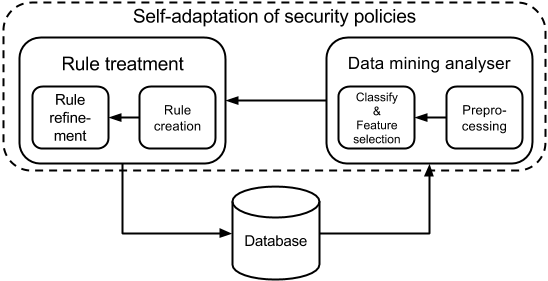
\includegraphics[width=0.5\textwidth]{./img/KRSgecco.png}
    \caption{Architecture overview of the proposed system, whith its inner components.}
    \label{fig:krs}
  \end{center}
\end{figure*}

\subsection{Data mining analyser}
\label{subsec:datamining}

This component wil be in charge of taking the desired `raw' data from the database, and processing it to remove errors or non-valid values, in order to obtain a dataset to be used in the rule treatment process. For instance, duplicated data or unknown values are considered as data that should be removed. Considered data corresponds to events (and their related information/context) produced by users' interactions with the system.
Then, the preprocessing component will be devoted to `prepare' this data for the application of further techniques such as pattern mining \cite{han2007frequent}. Patter mining allows the identification of non-frequent or anomalous patterns, since these are suspicious, and thus, could be of interest to be checked by the Chief Security Officer.

The next subcomponent performs tasks like feature selection \cite{guyon2003introduction}, which consists of choosing the most important data features/variables in order to reduce the dataset weight. Also, new features can be created by extracting meta-information from the existing ones. These two steps are mainly done for improving the performance of the classification stage. Then the subcomponent uses classification algorithms \cite{witten2005data}, i.e., it trains models (classifiers) able to associate every pattern in the dataset to a class. This way, the built classifier can assign a class to further incoming patterns.  In this case, the class will be the ``decision'' taken, which means that if the incoming user action is too similar to past dangerous patterns, it will be rejected ot denied.

\subsection{Rule treatment}
\label{subsec:ruletreatment}

This component will be focused in creating new rules and will also work with the existing CSPs.
It will globally perform three different tasks over them. First, it will take the set of classification rules from the previous component, and will merge or compare them with the existing ones, suggesting a first set of new (unrefined) rules. Then, it will analyse the existing rules in order to remove, from the created set in the first step, those which might be redundant. This is done for maintaining correctness and coherence in the system. Finally, taking advantage of the decision tree structure nature of the rules, the system will consider using Genetic Programming \cite{koza1992genetic}, as the kind of EA used for optimising tree-based structures. The final set of rules will be presented to the CSO of the company, then accept or reject them. This acceptance or rejection of rule process is itself a `feedback' from wich the system can learn.

%
%%%%%%%%%%%%%%%%%%%%%%%%%%%%%%% PRELIMINARY RESULTS %%%%%%%%%%%%%%%%%%%%%%%%%%%%%%%
%
\section{Preliminary Results}
\label{sec:results}

As mentioned, the decision of implementing this system is preceded by the result obtained in \cite{mora14:urls}. 

%
%%%%%%%%%%%%%%%%%%%%%%%%%%%%%%% CONCLUSIONS %%%%%%%%%%%%%%%%%%%%%%%%%%%%%%%
%
\section{Conclusions}
\label{sec:conclusions}

%
%%%%%%%%%%%%%%%%%%%%%%%%%%%%%%% ACKNOWLEDGEMENTS %%%%%%%%%%%%%%%%%%%%%%%%%%%%%%%
%
\section{Acknowledgements}

\bibliographystyle{plain}
\bibliography{sc_sec}

\end{document}
